\frame
{
\frametitle{Representaciones}
\begin{center}
	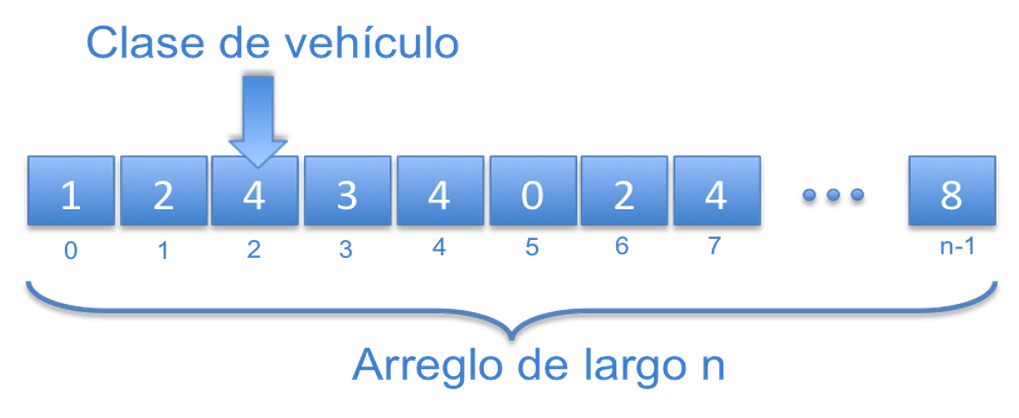
\includegraphics[width=0.7\textwidth]{img/representacion}
\end{center}
}

\frame
{
\frametitle{Representaciones}
\framesubtitle{Simulated Annealing}
\begin{itemize}
	\item Variables utilizadas
		\begin{itemize}
			\item {\tt T\_max:} Temperatura máxima.
        	\item {\tt N\_recal:} Número de recalentamientos.
			\item {\tt alpha:} Porcentaje de la temperatura máxima a recalentar.
			\item {\tt Delta\_t:} Temperatura a decrecer, el decrecimiento es aritmético.
			\item {\tt X:} Almacena la solución actual del problema, además se define {\tt x\_gen} y {\tt x\_opt}.
			\item {\tt Delta\_x:} Variación en la función objetivo.
		\end{itemize}
\end{itemize}
}

\frame
{
\frametitle{Representaciones}
\framesubtitle{Simulated Annealing}
\begin{itemize}
	\item Movimiento
	\begin{itemize}
		\item El movimiento escogido es el {\bf swap}, que realiza el cambio de dos variables.
		\item Este cambio se realiza al {\bf azar}, lo que genera una solución que será aceptada bajo las condiciones:
		\begin{itemize}
			\item Si es la función objetivo es menor que la actual, será aceptada.
			\item Si $P(0,1) \leq e^{-|delta_x|}$, será aceptada.
		\end{itemize}
	\end{itemize}
\end{itemize}
}

\begin{frame}[fragile]
\frametitle{Representaciones}
\framesubtitle{Simulated Annealing}
\tiny{
\begin{verbatim}
Inicio
t<-t_max // temperatura inicial
cont <- 0 // número de recalentamientos hechos
Leer Datos
solución<-Generar solución inicial
rest_h<-Contar restricciones violadas de solución
salir<-falso
rest<-rest_h
Mientras cont<numero
    rechazado<-falso
    Mientras rachazado=falso
        solución_gen<- Realizar movimiento a solución
        rest_gen<-Contar restricciones violadas de solución_gen
       	Verifica la aceptación
		Cambiar solución y rest por solución_gen y rest_gen si es mejor o es peor pero se acepta
        Cambiar solución_h y rest_h por solución_gen y rest_gen si es mejor
    Fin Mientras
    Decrecimiento de la temperatura   
    Si t<0 Entonces
        cont<-cont+1
        t<-t*alpha //alpha es una valor entre 0 y 1
    Fin Si
Fin Mientras
Imprimir Resultados
Fin
\end{verbatim}
}
\normalsize
\end{frame}

\frame
{
\frametitle{Representaciones}
\framesubtitle{Algoritmo Evolutivo + Simulated Annealing}
\begin{itemize}
	\item Aproximación a al representación matemática (fórmula).
	\item Estructuras de datos:
	\begin{itemize}
		\item Individuos (\texttt{{\bf struct} genotype}).
		\begin{itemize}
			\item {\tt{\bf int} gene[VARS]}, {\tt {\bf int} fitness}, {\tt {\bf int} fail}.
			\item {\tt {\bf double} rfitness}, {\tt {\bf double} cfitness}.
		\end{itemize}
	\end{itemize}
\end{itemize}
}

\frame
{
\frametitle{Representaciones}
\framesubtitle{Algoritmo Evolutivo + Simulated Annealing}
\begin{itemize}
	\item Estructuras de datos:
	\begin{itemize}
		\item Mejor Solución SA. ({\tt {\bf int} saBestSol[VARS]}).
		\item Número máximo de autos por subsecuencia.\\({\tt {\bf int} numMaxCarOptSeq[N]}).
		\item Tamaño de la subsecuencia. ({\tt {\bf int} sizeMaxCarOptSeq[N]}).
		\item Demanda y descripción de tipos de autos. ({\tt {\bf int} types[N][M]}).
	\end{itemize}
	\item Movimiento SA:
	\begin{itemize}
		\item {\bf swap}
		\item {\tt 10\% VARS}
	\end{itemize}
\end{itemize}
}

\begin{frame}[fragile]
\frametitle{Representaciones}
\framesubtitle{Algoritmo Evolutivo + Simulated Annealing}
\tiny{
\begin{verbatim}
Inicio
g <- 0 & p <- 0 // numero de generaciones y poblaciones
Leer datos de entrada
Población <- Generar población inicial
Evaluar población
    Mientras g < GENS
        Mientras n < POP - 1
            Selección individuo
            Mutación // Simulated Annealing + AM
        Fin Mientras
        Elitismo
        Cambio de población // Población actual = Población nueva
        Evaluar población
        n <- n + 1  &  p <- 0
    Fin Mientras
Imprimir resultados
Fin
\end{verbatim}
}
\normalsize
\end{frame}

